\documentclass[12pt]{article}
\author{GUILBERT Augustin, MARTINANT Valentin, OZDEMIR Serdar} 
\date{\today}
\title{\textsc{\textbf{Compression d'images}}}
\renewcommand{\baselinestretch}{1.2}
\usepackage{graphicx}
\usepackage[utf8]{inputenc} %accent
\usepackage[T1]{fontenc} %accent
\usepackage[frenchb]{babel} % choix de la langue 
\usepackage{graphicx} %inclure des images(PNG,JPG,PDF)
\usepackage{amsmath,amssymb}
\usepackage[top=2.5cm,bottom=2.5cm,left=2.5cm,right=2.5cm]{geometry} 
\usepackage{fancyhdr}
\usepackage{caption}
\pagestyle{fancy} 
\lfoot{TIPE Compression d'images} 
\rfoot{Lycée Blaise Pascal 2017-2018} 

\renewcommand{\footrulewidth}{0.8pt}

\begin{document}
\maketitle
\newpage
\tableofcontents
\newpage
\section{Objectifs et types de compression d'images}	
\subsection{Objectifs de la compression d'images}
Pour transférer des données numériques, un nombre plus ou moins importants de bits est utilisé. Le transfert d'image nécessite la mobilisation d'un très grand nombre de bits. C'est pourquoi l'image est compressée avant d'être transférée. La compression va permettre de réduire le nombre de données codant l'image, ainsi un moins grand nombre de données sera transféré ce qui permettra un transfert de l'image plus rapide.
\subsection{Types de compression d'images}
Comme dit précédemment, la compression d'image permet de réduire le nombre de données codant une image. Il existe deux grands types de compression: la compression avec perte et la compression sans perte.
\paragraph{}
		La compression sans perte est préférée quand la netteté des traits est primordiale ou vitale par exemple pour des schémas, des dessins techniques, balayages médicaux... La compression avec perte permet de réduire radicalement le nombre de données codant l'image, elle est utile pour des transmissions à bas débit mais dégrade souvent la qualité de l'image restituée. Cette méthode est préférée pour des photos dans les applications où une perte de fidélité (mineure bien sûr, et parfois imperceptible) peut être tolérée pour réduire les coûts de stockage ou d'envoi.
Dans la suite, nous parlerons uniquement de la compression (avec perte) DCT (Discrete Cosine Transform).

\newpage
\section{Compression JPEG}
Le format JPEG (Joint Photographic Experts Group) est un format d’image compressée qui offre une bonne compression pour une qualité très correcte. Ces deux avantages en font l’un des formats d’image les plus répandus, particulièrement sur le web où les problématiques de transfert et de stockage sont importantes.
Une image à laquelle on applique la compression JPEG suit le traitement suivant:
\paragraph{}
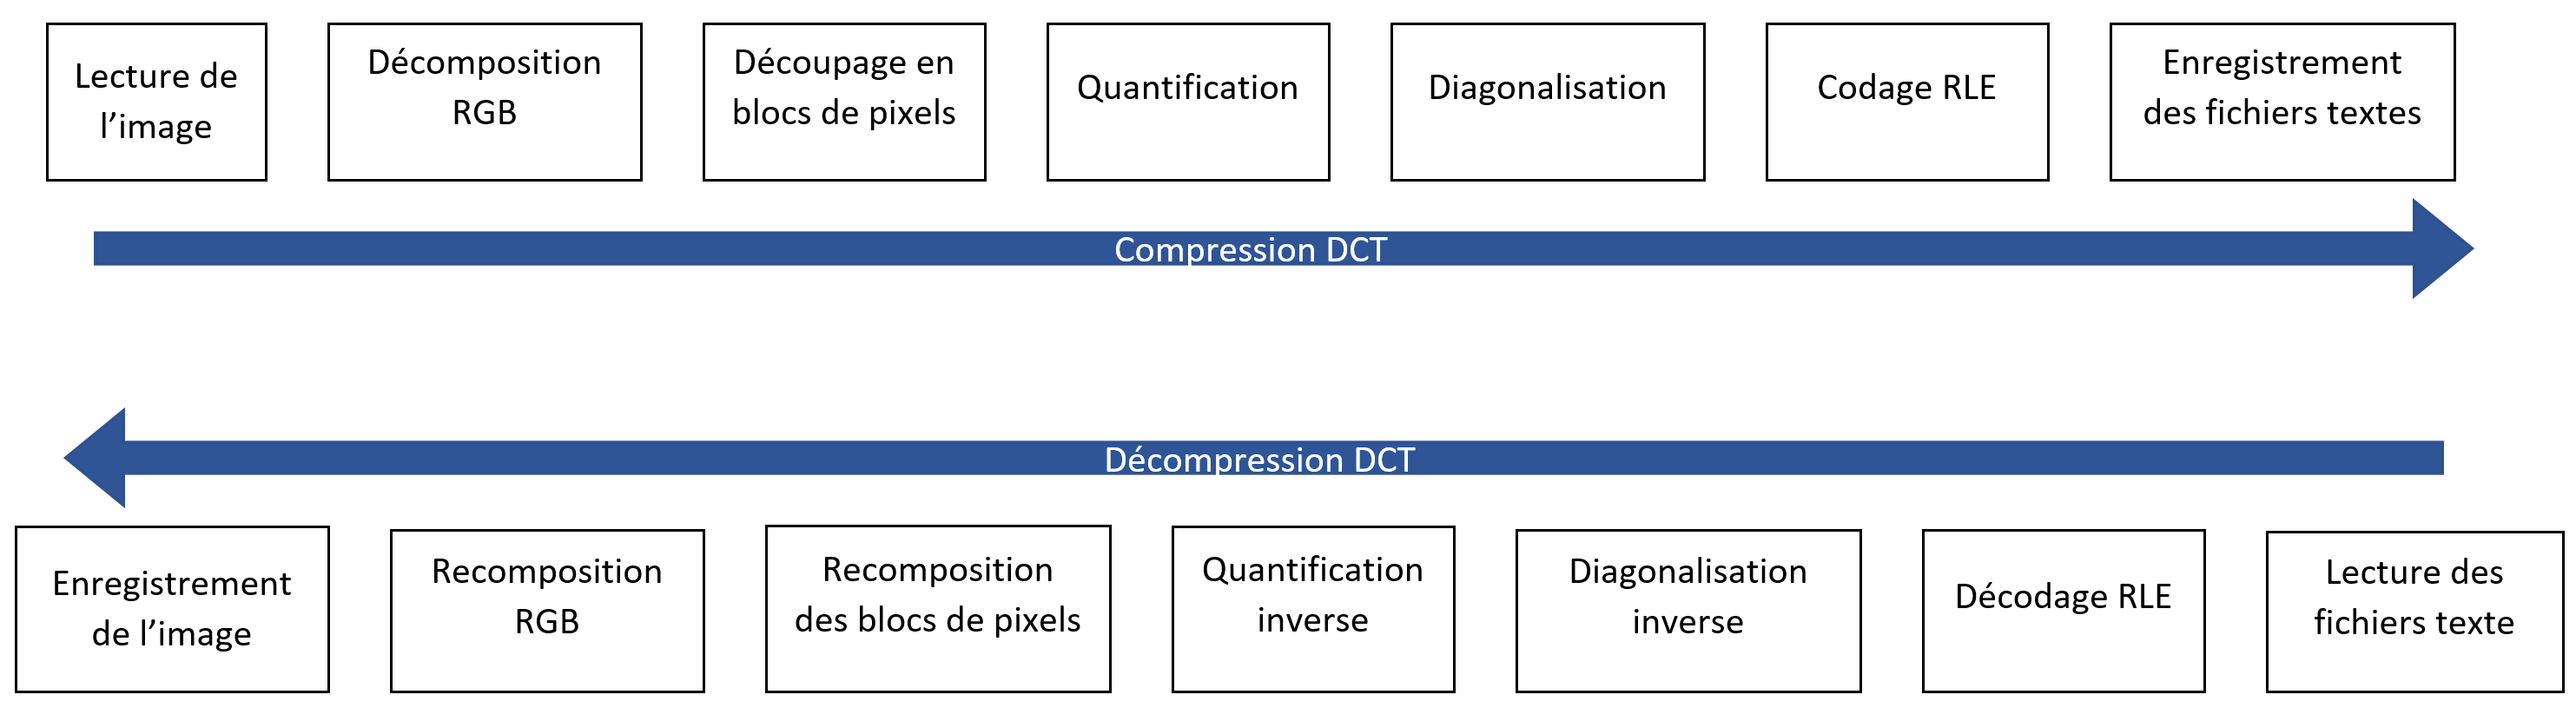
\includegraphics[scale=0.2]{schema_dct.png} %scale pour augmenter ou diminuer proportionnellement la hauteur et largeur de l'image


\begin{equation*} 
C(i)(j)=\cfrac{1}{\sqrt{2N}} \biggl[\sum_{1\leq x\leq N-1} \sum_{1\leq y\leq N-1} p(x,y) \cos{\biggl[\cfrac{(2x+1) i \Pi}{2N}}\biggr] \cos{\biggl[\cfrac{(2y+1) j \Pi}{2N}}\biggr]\biggr]
\end{equation*}
\begin{center}
$
\begin{Bmatrix}
.3536& .3536& .3536& .3536& .3536& .3536& .3536& .3536 \\
.4904& .4157& .2778& .0975& -.0975& -.2778& -.4157& -.4904 \\
.4619& .1913& -.1913& -.4619& -.4619& -.1913& .1913& .4619 \\
\end{Bmatrix}
$
\end{center}
\captionsetup{labelformat=empty}
\begin{table}[h]
\begin{center}
\begin{tabular}{|p{2,5cm}|p{3cm}|p{3,3cm}|p{2,5cm}|}
\hline
\centering Niveau de compression&\centering Taille originale (en Mo)&\centering Taille compressée (en Mo)&\centering Taux de compression\tabularnewline%\centering permet de centrer le contenue de la cellule suiante, il faut alors utiliser \tabularnawline pour sauter la ligne car \\ est désactivé
\hline
\centering 10&\centering 6,22&\centering 1,08&\centering 5,7\tabularnewline
\hline
\centering 20&\centering 6,22&\centering 1,26&\centering 4,9\tabularnewline
\hline
\centering 30&\centering 6,22&\centering 1,44&\centering 4,3\tabularnewline
\hline
\centering 40&\centering 6,22&\centering 1,60&\centering 3,9\tabularnewline
\hline
\centering 50&\centering 6,22&\centering 1,76&\centering 3,5\tabularnewline
\hline
\centering 60&\centering 6,22&\centering 1,90&\centering 3,3\tabularnewline
\hline
\centering 70&\centering 6,22&\centering 2,14&\centering 2,9\tabularnewline
\hline
\centering 80&\centering 6,22&\centering 2,56&\centering 2,4\tabularnewline
\hline
\centering 90&\centering 6,22&\centering 3,39&\centering 1,8\tabularnewline
\hline

\end{tabular}
\end{center}
\caption{Taux de compression en fonction du niveau de quantification choisi}
\end{table}

\

\end{document}
